\documentclass{standalone}
\usepackage{tikz}
\usetikzlibrary{patterns, positioning}

\begin{document}
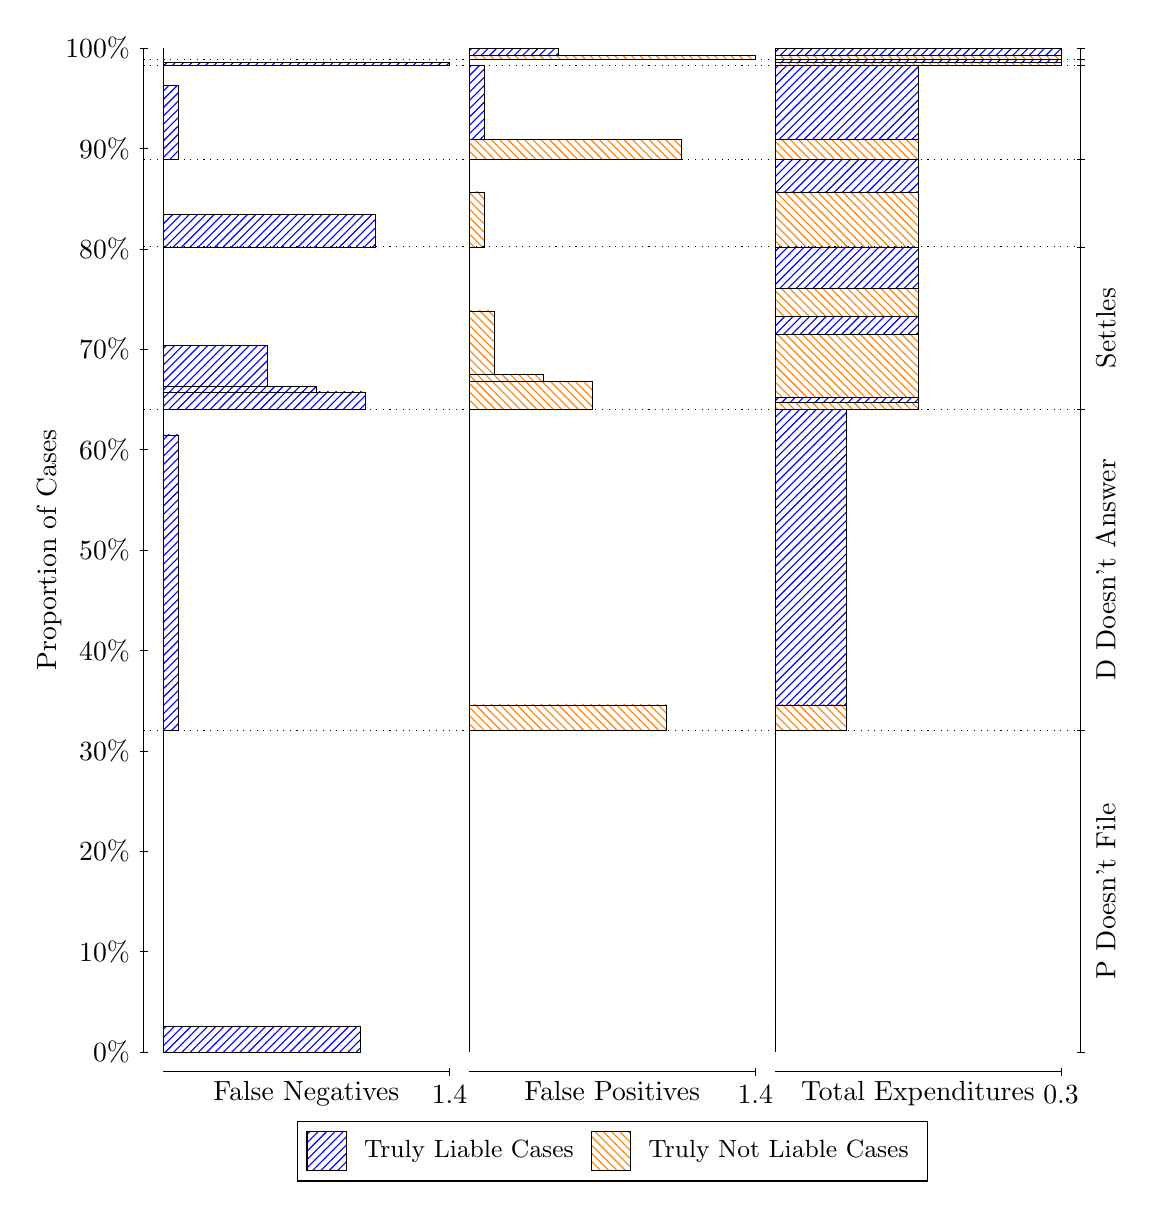
\begin{tikzpicture}
\draw[black, very thin] (1.5,1.75) -- (1.5,14.5);
\node[rotate=90, anchor=center] at (0.3, 8.125) {Proportion of Cases};
\draw[black, very thin] (1.45,1.75) -- (1.55,1.75);
\node[anchor=east] at (1.45, 1.75) {0\%};
\draw[black, very thin] (1.45,3.025) -- (1.55,3.025);
\node[anchor=east] at (1.45, 3.025) {10\%};
\draw[black, very thin] (1.45,4.3) -- (1.55,4.3);
\node[anchor=east] at (1.45, 4.3) {20\%};
\draw[black, very thin] (1.45,5.575) -- (1.55,5.575);
\node[anchor=east] at (1.45, 5.575) {30\%};
\draw[black, very thin] (1.45,6.85) -- (1.55,6.85);
\node[anchor=east] at (1.45, 6.85) {40\%};
\draw[black, very thin] (1.45,8.125) -- (1.55,8.125);
\node[anchor=east] at (1.45, 8.125) {50\%};
\draw[black, very thin] (1.45,9.4) -- (1.55,9.4);
\node[anchor=east] at (1.45, 9.4) {60\%};
\draw[black, very thin] (1.45,10.675) -- (1.55,10.675);
\node[anchor=east] at (1.45, 10.675) {70\%};
\draw[black, very thin] (1.45,11.95) -- (1.55,11.95);
\node[anchor=east] at (1.45, 11.95) {80\%};
\draw[black, very thin] (1.45,13.225) -- (1.55,13.225);
\node[anchor=east] at (1.45, 13.225) {90\%};
\draw[black, very thin] (1.45,14.5) -- (1.55,14.5);
\node[anchor=east] at (1.45, 14.5) {100\%};

\draw[black, very thin] (13.4,1.75) -- (13.4,14.5);
\draw[black, very thin] (13.35,1.75) -- (13.45,1.75);
\node[anchor=west] at (13.35, 1.75) {};
\draw[black, very thin] (13.35,5.832) -- (13.45,5.832);
\node[anchor=west] at (13.35, 5.832) {};
\draw[black, very thin] (13.35,9.9131) -- (13.45,9.9131);
\node[anchor=west] at (13.35, 9.9131) {};
\draw[black, very thin] (13.35,11.974) -- (13.45,11.974);
\node[anchor=west] at (13.35, 11.974) {};
\draw[black, very thin] (13.35,13.083) -- (13.45,13.083);
\node[anchor=west] at (13.35, 13.083) {};
\draw[black, very thin] (13.35,14.281) -- (13.45,14.281);
\node[anchor=west] at (13.35, 14.281) {};
\draw[black, very thin] (13.35,14.357) -- (13.45,14.357);
\node[anchor=west] at (13.35, 14.357) {};
\draw[black, very thin] (13.35,14.5) -- (13.45,14.5);
\node[anchor=west] at (13.35, 14.5) {};

\draw[black, very thin, pattern color=blue, pattern=north east lines] (1.75,1.75) rectangle (4.2557,2.0755);
\draw[black, very thin, pattern color=orange, pattern=north west lines] (1.75,2.0755) rectangle (1.75,5.832);
\draw[black, very thin, pattern color=blue, pattern=north east lines] (1.75,5.832) rectangle (1.9379,9.5881);
\draw[black, very thin, pattern color=orange, pattern=north west lines] (1.75,9.5881) rectangle (1.75,9.9131);
\draw[black, very thin, pattern color=blue, pattern=north east lines] (1.75,9.9131) rectangle (4.3184,10.132);
\draw[black, very thin, pattern color=blue, pattern=north east lines] (1.75,10.132) rectangle (3.692,10.198);
\draw[black, very thin, pattern color=blue, pattern=north east lines] (1.75,10.198) rectangle (3.0655,10.724);
\draw[black, very thin, pattern color=orange, pattern=north west lines] (1.75,10.724) rectangle (1.75,11.974);
\draw[black, very thin, pattern color=blue, pattern=north east lines] (1.75,11.974) rectangle (4.4437,12.384);
\draw[black, very thin, pattern color=orange, pattern=north west lines] (1.75,12.384) rectangle (1.75,13.083);
\draw[black, very thin, pattern color=blue, pattern=north east lines] (1.75,13.083) rectangle (1.9379,14.024);
\draw[black, very thin, pattern color=orange, pattern=north west lines] (1.75,14.024) rectangle (1.75,14.281);
\draw[black, very thin, pattern color=blue, pattern=north east lines] (1.75,14.281) rectangle (5.3833,14.318);
\draw[black, very thin, pattern color=orange, pattern=north west lines] (1.75,14.318) rectangle (1.75,14.357);
\draw[black, very thin, pattern color=orange, pattern=north west lines] (1.75,14.357) rectangle (1.75,14.407);
\draw[black, very thin, pattern color=blue, pattern=north east lines] (1.75,14.407) rectangle (1.75,14.5);
\draw[black, very thin, pattern color=orange, pattern=north west lines] (5.6333,1.75) rectangle (5.6333,5.5066);
\draw[black, very thin, pattern color=blue, pattern=north east lines] (5.6333,5.5066) rectangle (5.6333,5.832);
\draw[black, very thin, pattern color=orange, pattern=north west lines] (5.6333,5.832) rectangle (8.1391,6.157);
\draw[black, very thin, pattern color=blue, pattern=north east lines] (5.6333,6.157) rectangle (5.6333,9.9131);
\draw[black, very thin, pattern color=orange, pattern=north west lines] (5.6333,9.9131) rectangle (7.1994,10.271);
\draw[black, very thin, pattern color=orange, pattern=north west lines] (5.6333,10.271) rectangle (6.573,10.36);
\draw[black, very thin, pattern color=orange, pattern=north west lines] (5.6333,10.36) rectangle (5.9466,11.163);
\draw[black, very thin, pattern color=blue, pattern=north east lines] (5.6333,11.163) rectangle (5.6333,11.974);
\draw[black, very thin, pattern color=orange, pattern=north west lines] (5.6333,11.974) rectangle (5.8213,12.672);
\draw[black, very thin, pattern color=blue, pattern=north east lines] (5.6333,12.672) rectangle (5.6333,13.083);
\draw[black, very thin, pattern color=orange, pattern=north west lines] (5.6333,13.083) rectangle (8.327,13.34);
\draw[black, very thin, pattern color=blue, pattern=north east lines] (5.6333,13.34) rectangle (5.8213,14.281);
\draw[black, very thin, pattern color=orange, pattern=north west lines] (5.6333,14.281) rectangle (5.6333,14.32);
\draw[black, very thin, pattern color=blue, pattern=north east lines] (5.6333,14.32) rectangle (5.6333,14.357);
\draw[black, very thin, pattern color=orange, pattern=north west lines] (5.6333,14.357) rectangle (9.2667,14.407);
\draw[black, very thin, pattern color=blue, pattern=north east lines] (5.6333,14.407) rectangle (6.7609,14.5);
\draw[black, very thin, pattern color=orange, pattern=north west lines] (9.5167,1.75) rectangle (9.5167,5.5066);
\draw[black, very thin, pattern color=blue, pattern=north east lines] (9.5167,5.5066) rectangle (9.5167,5.832);
\draw[black, very thin, pattern color=orange, pattern=north west lines] (9.5167,5.832) rectangle (10.425,6.157);
\draw[black, very thin, pattern color=blue, pattern=north east lines] (9.5167,6.157) rectangle (10.425,9.9131);
\draw[black, very thin, pattern color=orange, pattern=north west lines] (9.5167,9.9131) rectangle (11.333,10.001);
\draw[black, very thin, pattern color=blue, pattern=north east lines] (9.5167,10.001) rectangle (11.333,10.067);
\draw[black, very thin, pattern color=orange, pattern=north west lines] (9.5167,10.067) rectangle (11.333,10.87);
\draw[black, very thin, pattern color=blue, pattern=north east lines] (9.5167,10.87) rectangle (11.333,11.089);
\draw[black, very thin, pattern color=orange, pattern=north west lines] (9.5167,11.089) rectangle (11.333,11.447);
\draw[black, very thin, pattern color=blue, pattern=north east lines] (9.5167,11.447) rectangle (11.333,11.974);
\draw[black, very thin, pattern color=orange, pattern=north west lines] (9.5167,11.974) rectangle (11.333,12.672);
\draw[black, very thin, pattern color=blue, pattern=north east lines] (9.5167,12.672) rectangle (11.333,13.083);
\draw[black, very thin, pattern color=orange, pattern=north west lines] (9.5167,13.083) rectangle (11.333,13.34);
\draw[black, very thin, pattern color=blue, pattern=north east lines] (9.5167,13.34) rectangle (11.333,14.281);
\draw[black, very thin, pattern color=orange, pattern=north west lines] (9.5167,14.281) rectangle (13.15,14.32);
\draw[black, very thin, pattern color=blue, pattern=north east lines] (9.5167,14.32) rectangle (13.15,14.357);
\draw[black, very thin, pattern color=orange, pattern=north west lines] (9.5167,14.357) rectangle (13.15,14.407);
\draw[black, very thin, pattern color=blue, pattern=north east lines] (9.5167,14.407) rectangle (13.15,14.5);
\draw[black, dotted] (1.5,5.832) -- (13.4,5.832);
\draw[black, dotted] (1.5,9.9131) -- (13.4,9.9131);
\draw[black, dotted] (1.5,11.974) -- (13.4,11.974);
\draw[black, dotted] (1.5,13.083) -- (13.4,13.083);
\draw[black, dotted] (1.5,14.281) -- (13.4,14.281);
\draw[black, dotted] (1.5,14.357) -- (13.4,14.357);
\draw[black, very thin] (1.75,1.5) -- (5.3833,1.5);
\node[anchor=north] at (3.5667, 1.5) {False Negatives};
\draw[black, very thin] (5.3833,1.45) -- (5.3833,1.55);
\node[anchor=north] at (5.3833, 1.45) {1.4};

\draw[black, very thin] (5.6333,1.5) -- (9.2667,1.5);
\node[anchor=north] at (7.45, 1.5) {False Positives};
\draw[black, very thin] (9.2667,1.45) -- (9.2667,1.55);
\node[anchor=north] at (9.2667, 1.45) {1.4};

\draw[black, very thin] (9.5167,1.5) -- (13.15,1.5);
\node[anchor=north] at (11.333, 1.5) {Total Expenditures};
\draw[black, very thin] (13.15,1.45) -- (13.15,1.55);
\node[anchor=north] at (13.15, 1.45) {0.3};

\node[black, centered, rotate=90] at (13.72, 3.791) {P Doesn't File};
\node[black, centered, rotate=90] at (13.72, 7.8725) {D Doesn't Answer};
\node[black, centered, rotate=90] at (13.72, 10.943) {Settles};





\draw (7.449999999999999,1.5) node[draw=none] (baseCoordinate) {};
\begin{scope}[align=center]
        \matrix[scale=0.5, draw=black, below=0.5cm of baseCoordinate, nodes={draw}, column sep=0.1cm]{
            \node[rectangle, draw, minimum width=0.5cm, minimum height=0.5cm, pattern=north east lines, pattern color=blue] {}; &
            \node[draw=none, font=\small] (B) {Truly Liable Cases}; &
            \node[rectangle, draw, minimum width=0.5cm, minimum height=0.5cm, pattern=north west lines, pattern color=orange] {}; &
            \node[draw=none, font=\small] (B) {Truly Not Liable Cases}; \\
            };
\end{scope}

\end{tikzpicture}
\end{document}